

\section{Methods}

% brief outline of the section
\noindent The following section is organized as follows. First, we introduce a formalization of general problem setting, together with the variants considered in this work. Then, we outline the architecture of our model and how it can be mapped to neurobiology. Finally, we describe the learning procedure,
and showcase its dynamics in a simple example.


% mathematical formulation of the k-armed bandit problem.
\subsection{Binomial K-armed bandit problem}
\hfill \break
\noindent The standard formulation of the task is structured as a set of $K$ arms (or levers) $\mathcal{A}_{K}=\{a_{1}\ldots a_{K}\}$, with an associated reward distribution $\mathbf{p}=\{p_{1}, \ldots p_{K}\}$.
At each iteration, the agent pulls an arm and collects a possible reward drawn as a Bernoulli variable $R\sim \mathcal{B}(\{0,1\},p_{k})$. The agent's objective is maximizing the total reward $\sum^{T}_{t} R_{t}$, after a certain number $T$ of rounds, also called horizon.
Importantly, the agent is unaware of the true reward probabilities, and thus has to make its decisions following a certain policy, denoted as $\pi$.
In the reinforcement learning literature, the policy is often defined as a distribution over actions, here the arms $\mathcal{A}_{K}$, given the current state at time $t$. In the bandit problem, the state can be taken to correspond to the history $h_{t}$ of past actions and rewards in the period
$(0\ldots t]$, and the policy as a function that return a selected arm $\pi(h_{t})=a_{t}$ \cite{qiForcedExplorationBandit2023}.

Given the inherent stochasticity of the feedbacks from the environment, the policy is affected by the so-called exploration-exploitation trade-off, which here is phrased as the contrast between the option of the arm with the estimated highest expected reward versus the option to explore other arms, so to gather more information.
A common approach is the $\epsilon-$greedy policy, where the choice to explore is selected with a probability $\epsilon$.
Moreover, it is often preferable to have a more explorative behaviour early during the training, with the intent to have a good sample size for the empirical reward distribution, which can be later exploited for maximizing reward.

% regret
Another important concept in multi-armed bandit problems is \textit{regret}. Intuitively, it is defined as the deviation of the total reward obtained by the agent from the optimal reward that could have been obtained by always choosing the arm with the highest expected reward.
Formally, for a stationary distribution\footnote{\textbf{<<NB>>} should I generalize to non-stationary distribution, e.g. using extected values?} the regret is defined as:
\begin{equation}
    \rho=R^{*} - \sum^{T}_{t} R_{t}
\end{equation}

\noindent where $R^{*}$ is the reward obtained by always choosing the arm $a_{k}$ associated with the highest expected reward: $R^{*}=T\max_{k}\{\mathbf{p}\}$, and $R_{t}$ is the empirical reward obtained up to time $t$ by following policy $\pi$: $R_{t}=\sum^{T}_{t=1}\mathcal{B}(\pi(h_{t}))$.
The regret is a measure of the performance of the agent, and it is often used to compare different algorithms. The goal of the agent is to minimize the regret, and thus maximize the total reward.

% minimal model description

\subsection{Model description}
The model is constructed as a rate network of two populations of neurons \textit{M} and \textit{P}, the former representing the memory trace of the \textit{K} available options (\textit{i.e.} the bandits), and the latter representing the value of the options under the current policy.
More formally, the model is described by a set of coupled ordinary differential equations (ODEs) that capture the decision-making process in two distinct neural spaces.
The first equation tracks the evolution of the neural activity $\textbf{u}$ of \textit{M}, while the second tracks the activity $\textbf{v}$ of the \textit{P}. The time constants $\tau$ are the same for both equations and are set to $\tau = 10$ ms.


\begin{equation}
\begin{aligned}
    \tau \dot{\textbf{u}}&= -\textbf{u} + \textbf{v} + \textbf{I}_{\text{ext}} \\
    \tau \dot{\textbf{v}}&= -\textbf{v} + \textbf{z} \odot\textbf{u}
\end{aligned}
\end{equation}

\noindent The external input $\textbf{I}_{\text{ext}}$ is a constant input that is used to set the initial conditions of the neural activity $\textbf{u}$.
The term $\textbf{z}$ is a vector that weights the contribution of the active options $\textbf{u}$ to the value representation $\textbf{v}$, and functionally it is the core of the policy adopted by the model.
In practice, $\textbf{z}$ defined as a function of the synaptic weights $\textbf{W}^{MP}$ from \textit{M} to \textit{P} as $\textbf{z} = \Phi_v(\textbf{W}^{MP})$. Importantly, the connections are not fully connected, but rather are simply one-to-one mapping between the corresponding neurons in each
population, such that the weight matrix $\textbf{W}^{MP}$ is simply a matrix $K\times 1$, namely a vector.
The function $\Phi_v$ is a chosen to be a sum of a generalized sigmoid and a Gaussian, whose contributions are weighted by a parameter $r$:

\begin{equation*}
    \Phi_v(x) = r\gamma_{1} \frac{1}{1 + e^{-\beta(x-\alpha)}} + (1-r)\gamma_{2} \exp\left(-\frac{(x-\mu)^2}{2\sigma^2}\right)
\end{equation*}

\noindent The motivation behind this choice is to express a function that possesses a bounded region (depending on $\mu,\,\sigma$) at a high/low peak (depeding on the value of $\gamma_{2}$), and a continuous transition to a constant value (depending on the steepness of the sigmoid $\beta$, shift
$\alpha$, and intensity $\gamma_{1}$).

\hfill \break
\textbf{Option selection} \\
The decision-making process within a single round is structured in two distinct phases. Initially, the model receives a constant external input targeting all neurons in the memory population \textit{M} equally.
During this phase, $I_{\text{ext}}$ works as an equilibrium value while the reciprocal interactions with population \textit{P} push $\textbf{u}$ to different values, depending on the current policy encoded in $\textbf{z}$. However, in the early rounds the weights $\textbf{W}^{MP}$ are zero, and thus
the contribution from \textit{P} is null. After a fixed amount of time $\sim 5 \text{s}$, the second phase begins. Here, the external input is removed and the model is left to evolve autonomously, and since there are no recurrent connections in neither population the dynamics is entirely driven by their coupling. \\
A selection $\hat{k}$ is sampled after another fixed amount of time $\sim 5 \text{s}$, and it is defined according to the following rule:

\begin{equation*}
    \hat{k} =
    \left\{
        \begin{array}{ll}
            \text{argmax}_{k}\{\textbf{v}\} & \text{\textit{if}}\; \text{argmax}_{k} \{\textbf{v}\} = \text{argmax}_{k} \{\textbf{u}\} \\
            \text{random}(K) & \text{\textit{otherwise}}
        \end{array}
    \right.
\end{equation*}

\noindent The selection rule is simple: if the value representation $\textbf{v}$ is in agreement with the memory trace $\textbf{u}$, then the option with the highest value is selected. Otherwise, a random option is chosen. This rule is a way to express the exploration-exploitation trade-off, and it is dependent on the current policy $\textbf{z}$.

\hfill \break
\textbf{Learning} \\
Given a selected option, the environment (bandit) samples and returns a reward $R\in [0, 1]$.
Then, the connections $\textbf{W}^{MP}$ for the neuron corresponding to the option $k$ are updated according to the following plasticity rule:

\begin{equation}
    \Delta \textbf{W}^{MP}_{k} = \tilde{\eta}_{k} \left(R\cdot W^{+}- \textbf{W}^{MP}_{k}\right)
\end{equation}

\noindent
Where $W^{+}$ is a constant value that sets the upper bound for the synaptic weights, and it is set to $W^{+} = 5$, while $\tilde{\eta}_{k}$ is the learning rate for the option $k$ determined by a function of the current weights $\textbf{W}^{MP}_{k}$ and its shape is the same as $\Phi_{v}$, but with
different parameters.




% Evolution: fitness evolution
\subsection{Evolution search}
The optimization of the hyper-parameters was performed using the Covariance Matrix Adaptation evolutionary strategy algorithm (CMA-ES) \cite{igelCovarianceMatrixAdaptation2007}.
The search was run with a population of $256$ individuals (unique set of genomes corresponding to a sample in parameter space) for $40$ generations. The fitness function was defined as the average reward obtained by an individual over 2 independent iterations.
The results are summarized below in figure \ref{fig:evolution}.

\begin{figure}[H]
    \centering
    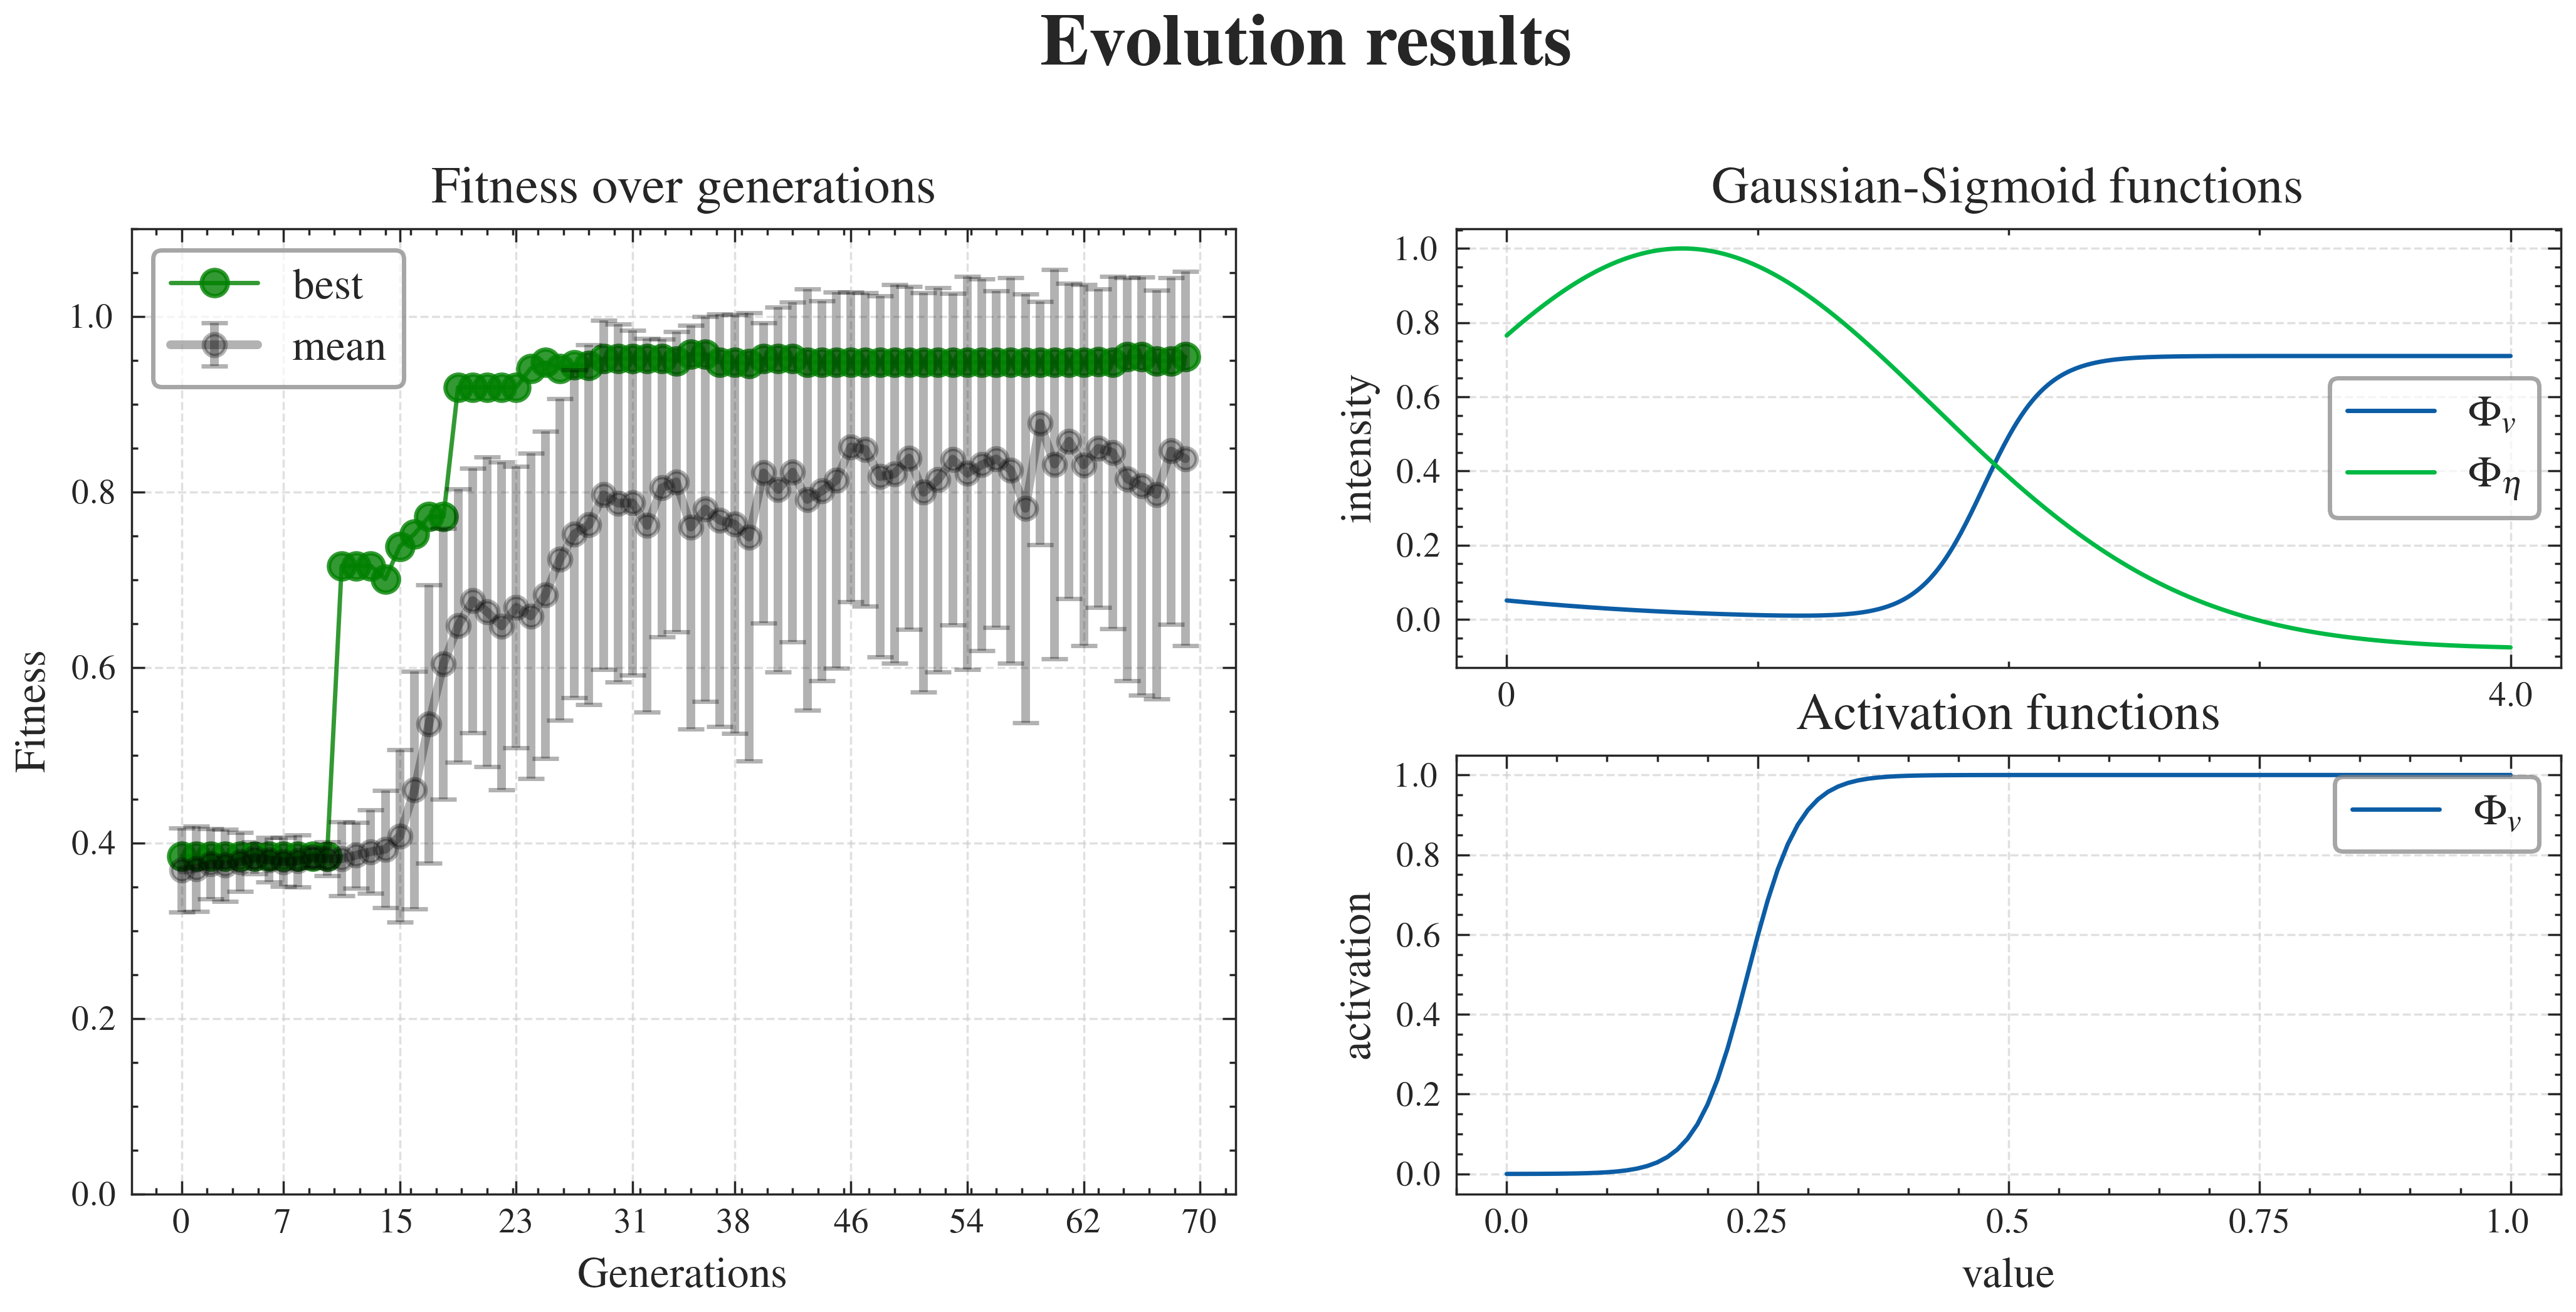
\includegraphics[width=1.0\textwidth]{figures/evolution_plot.png}
    \caption{\textsc{Evolution of the model over generations.} - Left: \textit{top fitness, mean and standard deviation (16-84 percentile) of the population over generations.} - Top-Right: \textit{option value and learning rate Gaussian sigmoid functions parametrized according to the genome of the fittest individual}
    Bottom-Right: \textit{activation function for population $v$ and $u$}}
    \label{fig:evolution}
\end{figure}

% comment on the evolved functions
\noindent The evolution results show a steady improvement of the fitness over generations, before hitting a plateau corresponding to the theoretical optimal ($\sim 0.9$) of the chosen simulations.

\textbf{TELL ME ABOUT THE RESPONSE FUNCTIONS, LIKE IS IT A TYPE II NEURON FR?} Regarding the evolved functions, the option value function $\Phi_{v}$ is characterized by a steep sigmoid curve, with a marked.
This is consistent with the idea that the input of population $U$ to population $V$ is weighted maximally for high option values (strong synapses), whereas for weaker estimates the contributions are low or close to zero, allowing for more exploration.

The learning rate function $\Phi_{\eta}$ is instead characterized by a marked bell-shaped curve, given a parameter $r=0.06$. The associated Gaussian has a positive mean located at $\mu=1.$, which aligns approximately with the local valley of the weight function $\Phi_{v}$.
A possible interpretation is that it serves as a mechanism to ensure that the learning rate is high when the value options are more uncertain, and low otherwise, thus preventing overshooting and oscillations in the weight updates.
This adaptive behaviour is in line with known neuronal dynamics such as homeostatic plasticity, which works towards a stabilization of synapses, for instance through synaptic scaling and proportional updates \cite{citriSynapticPlasticityMultiple2008}.
A variable learning rate is an important feature of several plasticity rules, from the more biologically plausible like the Oja \cite{ojaOjaLearningRule2008} to deep learning optimizers like Adam \cite{kingmaAdamMethodStochastic2017}.


\subsection{Bio-inspired features}

The model is inspired by the functioning of the prefrontal cortex (PFC) and its importance in decision-making processes. In particular, the two population $U, V$ of the model can be related to the orbito-frontal cortex (OFC) and anterior cingulate cortex (ACC), respectively.
More specifically, the OFC is known to be involved in the representation of the state different options and update their value with respect to rewarding outcomes and their history \cite{lukChoiceCodingFrontal2013, kennerleyDecisionMakingReward2011a}.
The ACC has been associated to action values and influencing the exploration-exploitation assessment \cite{khamassiChapter22Medial2013}. Further, its dynamic interplay with the OFC is observed to elicit transient pre-stimulus activation, which biases the decision towards the most valuable option \cite{funahashiPrefrontalContributionDecisionMaking2017, marcosDeterminingMonkeyFree2016, balewskiValueDynamicsAffect2023}.

In the model, the first layer represents the available options, while the learned connections with the second layer encode their values based on the recent reward history.
Another similarity with this particular pre-frontal circuit is the realization of a choice as a sample of the network state after a period of autonomous neural activity, where the stability of the neural activations depend on the strength and reliability of the highest option value \cite{backmanEffectsWorkingMemoryTraining2011, enelStableDynamicRepresentations2020}.
Moreover, the application of the function $\Phi_{v}$ on the connections $\textbf{W}^{UV}$ can be regarded as meta-plasticity, mediated by a neuromodulator \cite{wangMetalearningNaturalArtificial2021}.

